\documentclass[12pt]{article}
\usepackage[T1]{fontenc}
\usepackage[T1]{polski}
\usepackage[utf8]{inputenc}
\usepackage{graphicx}
\usepackage{amsfonts}
\usepackage{float}

\setlength{\textheight}{20cm}

\title{{\bf Zadanie nr 3 - Splot, filtracja i korelacja sygnałów}\linebreak
Cyfrowe Przetwarzanie Sygnałów}
\author{Krzysztof Barden, 210139 \and Paweł Galewicz, 210182}
\date{17.05.2019r.}

\begin{document}
\clearpage\maketitle
\thispagestyle{empty}
\newpage
\setcounter{page}{1}
\section{Cel zadania}

Celem ćwiczenia jest zaimplementowanie:
\begin{itemize}
\item operacji splotu dysktretnego dla dowolnychh dwóch sygnałów dyskretnych o arbitralnie podanych ilosciach próbek,
\item filtrów o skończonej odpowiedzni SOI (ang. FIR - Finite Impulse Response) - dolnoprzepustowego, górnoprzepustowego i pasmowego,
\item korelacji wzajemnej dla dowolnych dwóch sygnałów dyskretnych o arbitralnie podanych ilosciach próbek implementując bezposrednio oraz z użyciem splotu,
\item symulacji działania korelacyjnego czujnika odległosci (anteny).
\end{itemize}

\section{Wstęp teoretyczny}

Program z zadania 1 i 2 został rozszerzony o dodadtkowe funkcjonalnosci. Wykresy generowane są przy użyciu biblioteki LiveCharts \cite{lv}. GUI aplikacji zostało stworzone przy użyciu biblioteki WPF \cite{wpf}.
\\Interfejs został rozszerzony o interfejs anteny:
\begin{figure}[H]
 \centering
 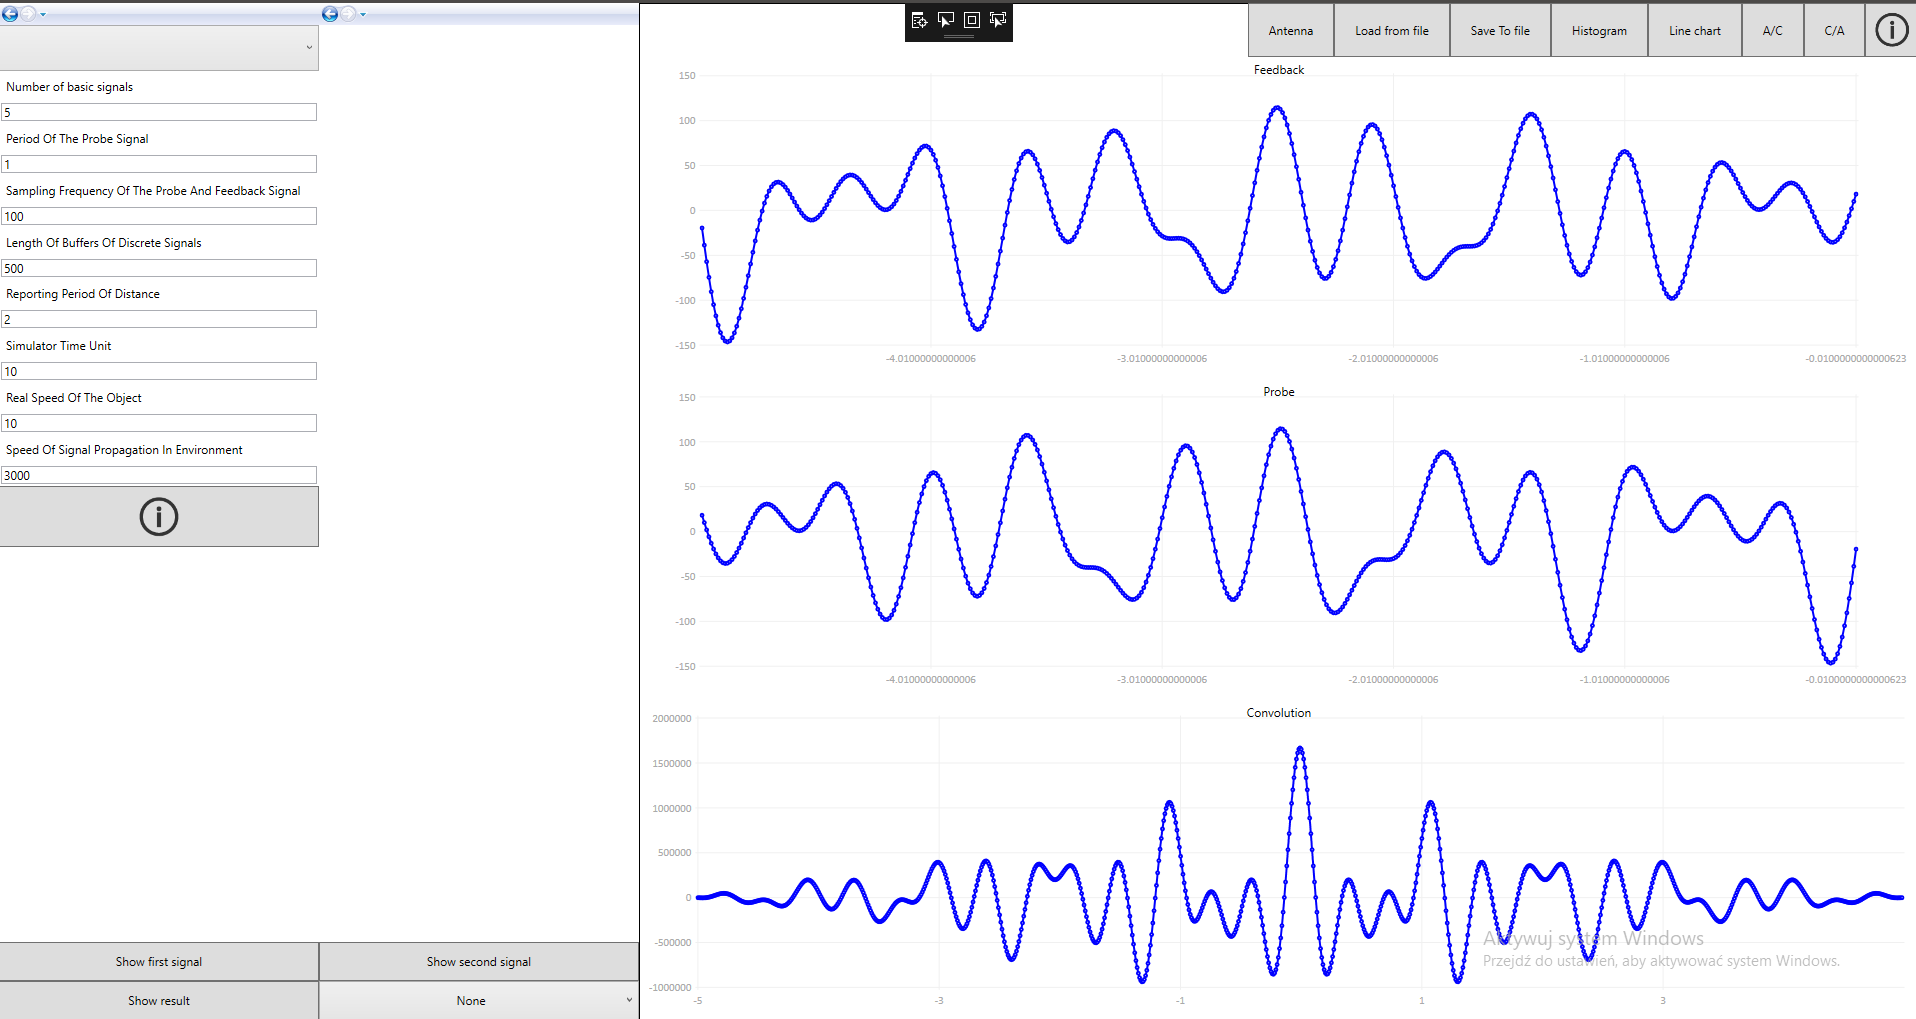
\includegraphics[width=15cm]{images/gui1.PNG}
 \vspace{-0.3cm}
 \caption{Interfejs graficzny anteny}
 \label{gui}
\end{figure}

Aby wygenerować sygnały należy w lewej kolumnie wypełnić parametry i nacisnąć przycisk "i". 
\section{Eksperymenty i wyniki}


%%%%%%%%%%%%%%%%%%%%%%%%%%%%%%%%%%%%%%%%%%%%%%%%%%%%%%%%%%%%%%%%%%%%%%%%%%%%%%%%%%%%%%%%%%%%%%%%%%%%%%%%%%%%%%%%%
% PODROZDZIAŁ PT. EKSPERYMENT NR 1 
%%%%%%%%%%%%%%%%%%%%%%%%%%%%%%%%%%%%%%%%%%%%%%%%%%%%%%%%%%%%%%%%%%%%%%%%%%%%%%%%%%%%%%%%%%%%%%%%%%%%%%%%%%%%%%%%%

Do zaprezentowania możliwosci korelacyjnego czujnika odległosci przedstawimy eksperyment w którym dokonamy pomiarów dla 3 sygnałów, każdy z innymi parametrami sygnałów.

\subsection{Eksperyment nr 1 }
\subsubsection{Korelacyjny czujnik odległosci}
Celem tego eksperymentu było wygenerowanie szumu o rozkladzie jednostajnym.


\subsubsection{Rezultat}

\begin{figure}[H]
 \centering
 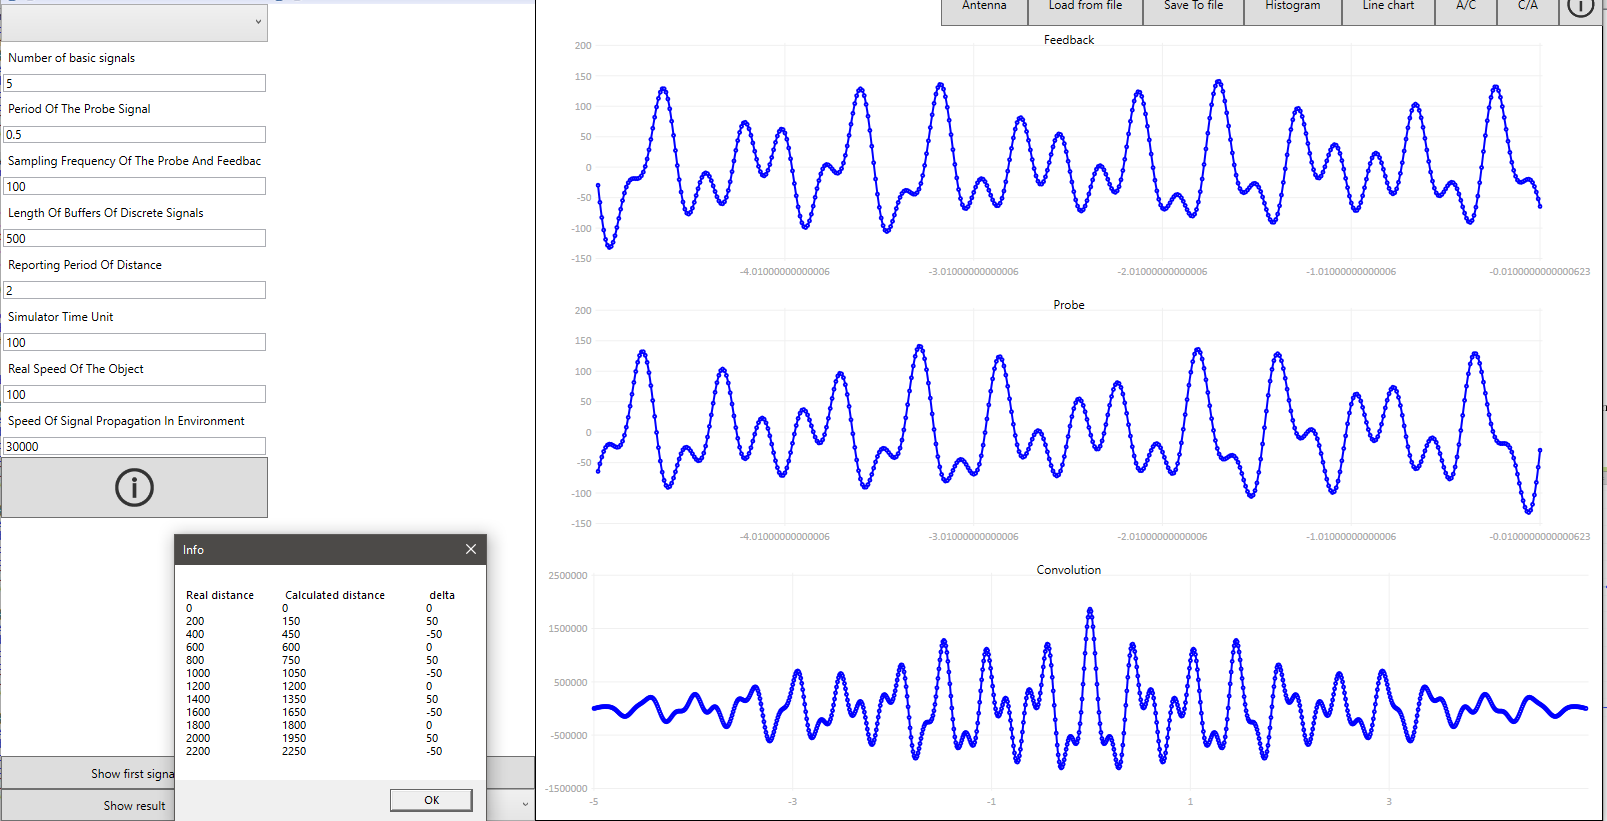
\includegraphics[width=14cm]{images/a1.PNG}
 \vspace{-0.3cm}
 \caption{Wykres szumu o rozkladzie jednostajnym}
 \label{gui}
\end{figure}

\begin{figure}[H]
 \centering
 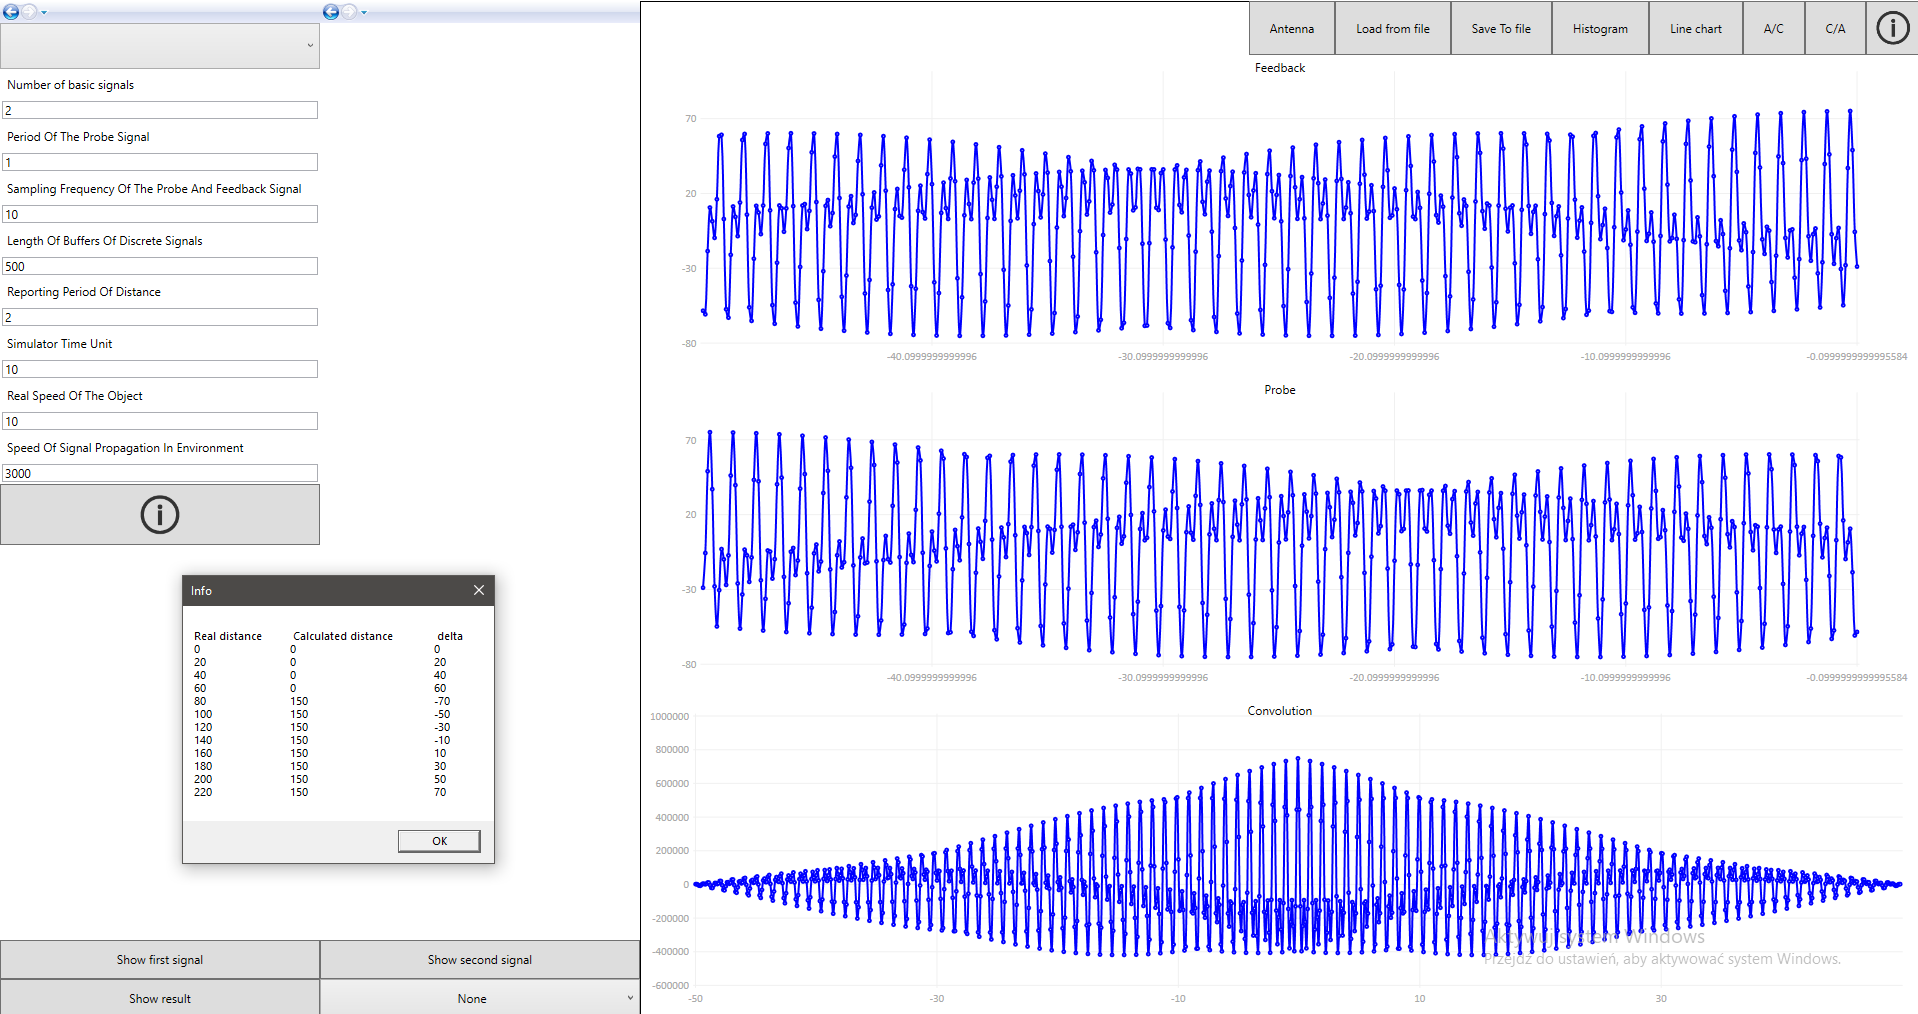
\includegraphics[width=14cm]{images/a2.PNG}
 \vspace{-0.3cm}
 \caption{Korelacyjny czujnik odległosci}
 \label{gui}
\end{figure}


\begin{figure}[H]
 \centering
 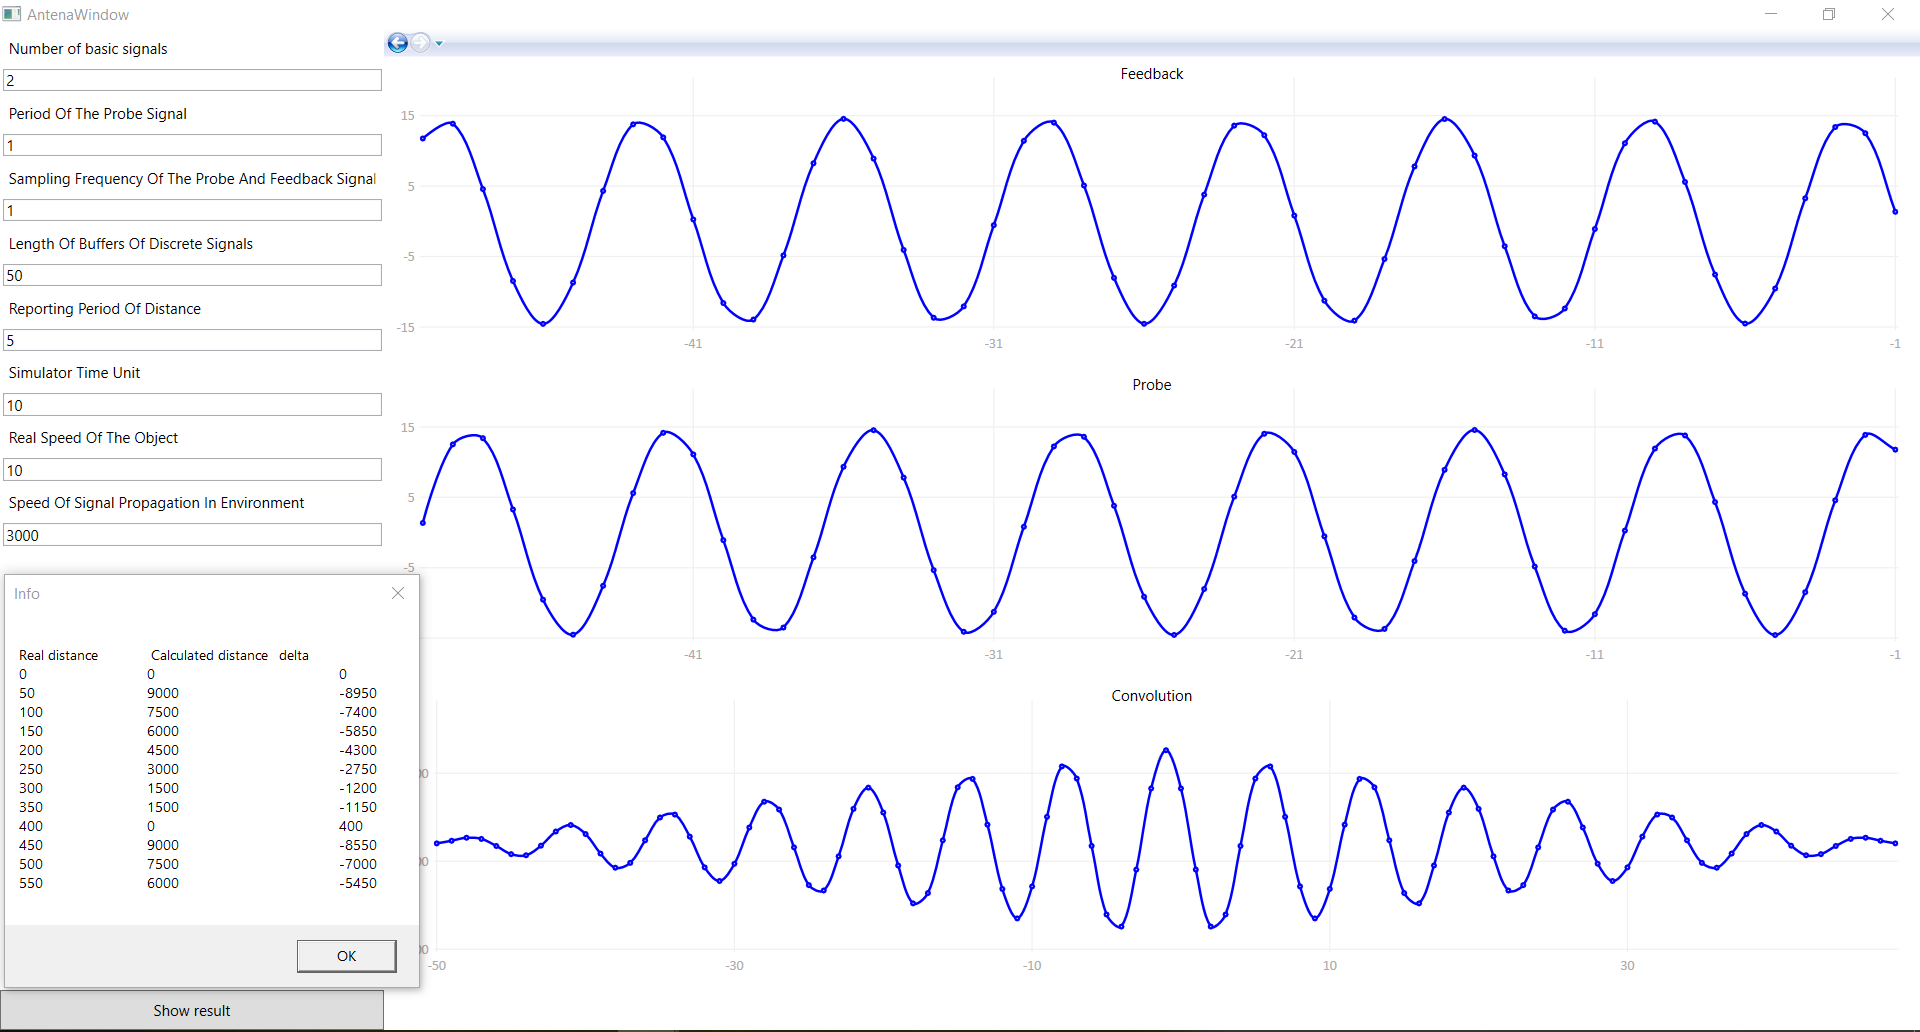
\includegraphics[width=14cm]{images/a3.PNG}
 \vspace{-0.3cm}
 \caption{Korelacyjny czujnik odległosci}
 \label{gui}
\end{figure}




%%%%%%%%%%%%%%%%%%%%%%%%%%%%%%%%%%%%%%%%%%%%%%%%%%%%%%%%%%%%%%%%%%%%%%%%%%%%%%%%%%%%%%%%%%%%%%%%%%%%%%%%%%%%%%%%%
% PODROZDZIAŁ PT. EKSPERYMENT NR 2
%%%%%%%%%%%%%%%%%%%%%%%%%%%%%%%%%%%%%%%%%%%%%%%%%%%%%%%%%%%%%%%%%%%%%%%%%%%%%%%%%%%%%%%%%%%%%%%%%%%%%%%%%%%%%%%%%


\subsection{Eksperyment nr 2 }
\subsubsection{Generowanie sygnału sinusoidalnego wyprostowanego jednopołówkowo}
Celem tego eksperymentu było wygenerowanie szumu o rozkladzie jednostajnym.


\subsubsection{Rezultat}

\begin{figure}[H]
 \centering
 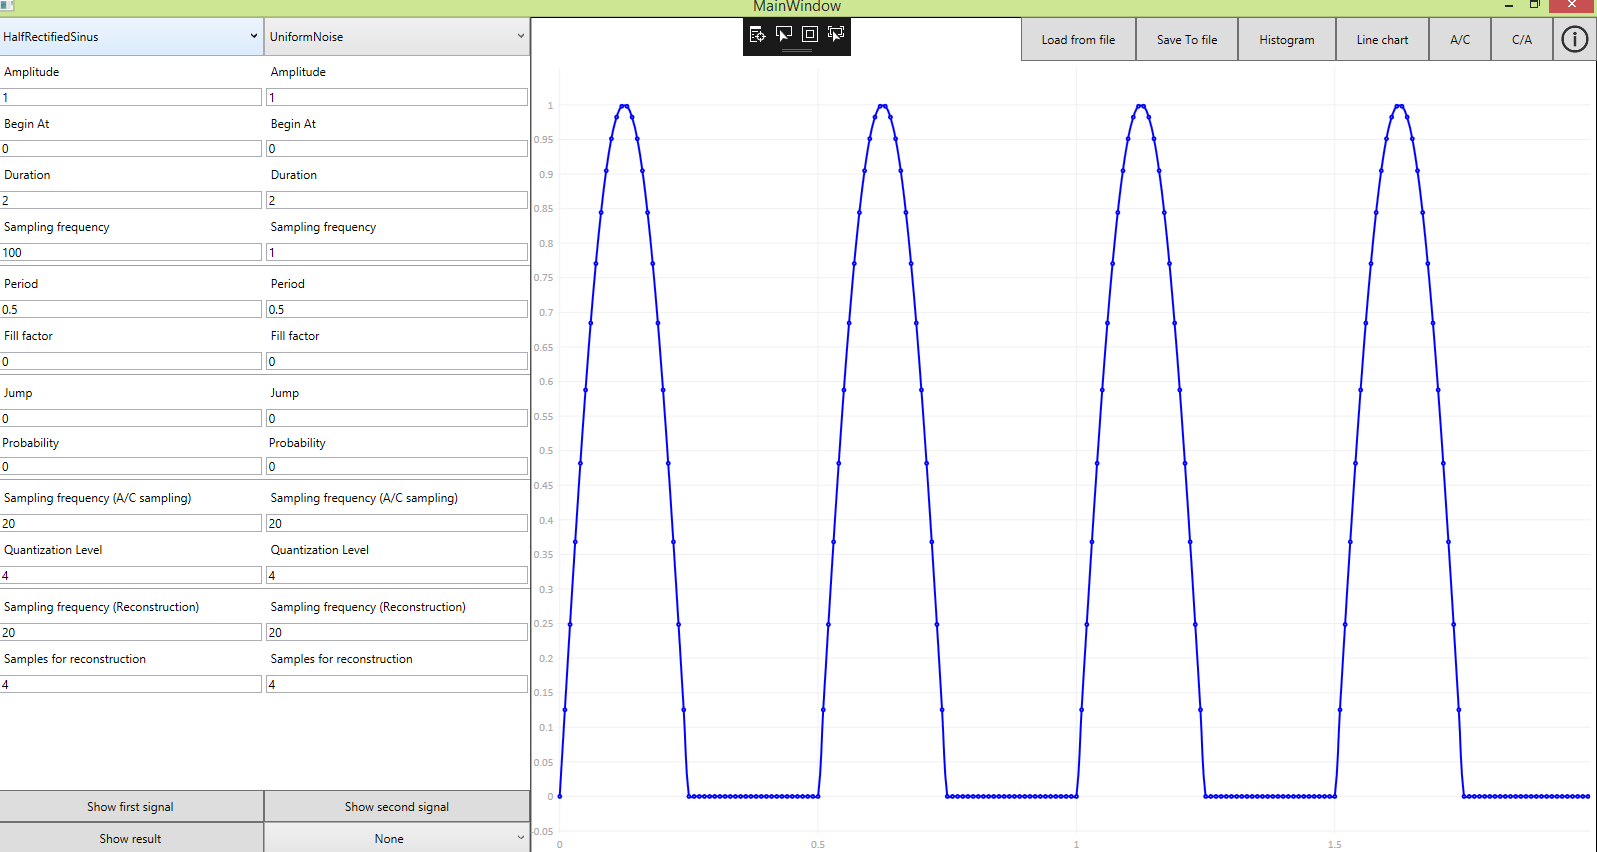
\includegraphics[width=14cm]{images/hsinline.PNG}
 \vspace{-0.3cm}
 \caption{Wykres sygnału sinusoidalnego wyprostowanego jednopołówkowo}
 \label{gui}
\end{figure}

\begin{figure}[H]
 \centering
 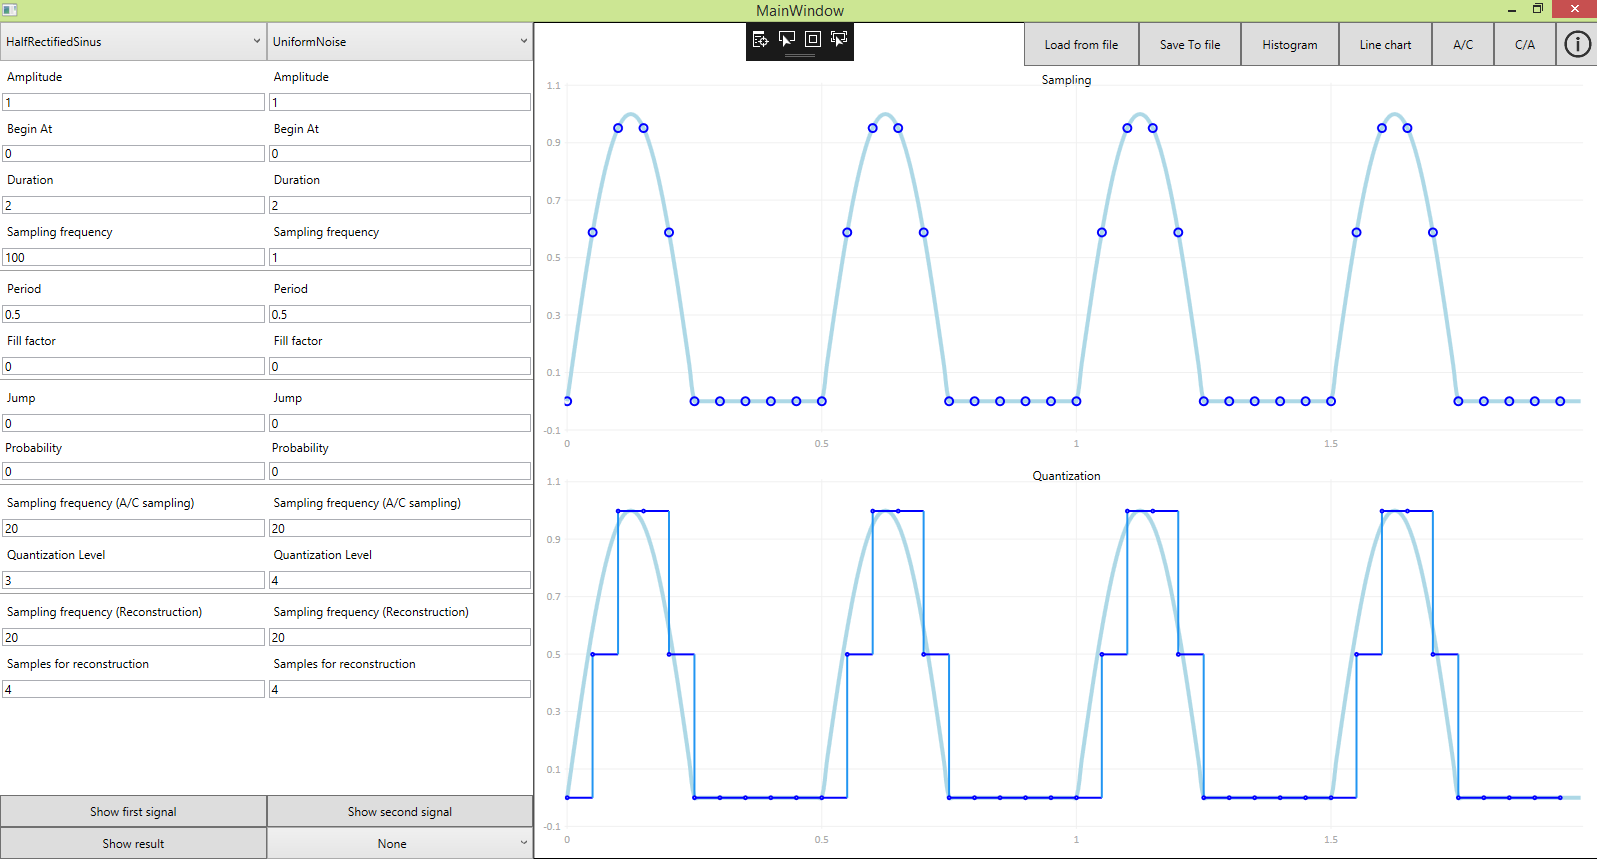
\includegraphics[width=14cm]{images/hsinac.PNG}
 \vspace{-0.3cm}
 \caption{Konwersja A/C , poziom kwantyzacji = 4}
 \label{gui}
\end{figure}

\begin{figure}[H]
 \centering
 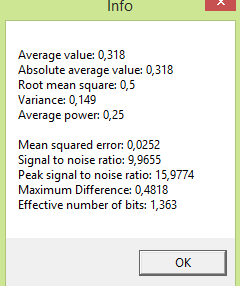
\includegraphics[width=7cm]{images/hsininfo.PNG}
 \vspace{-0.3cm}
 \caption{Wyliczone wartosci dla sygnału sinusoidalnego wyprostowanego jednopołówkowo  , poziom kwantyzacji = 4}
 \label{gui}
\end{figure}

\begin{figure}[H]
 \centering
 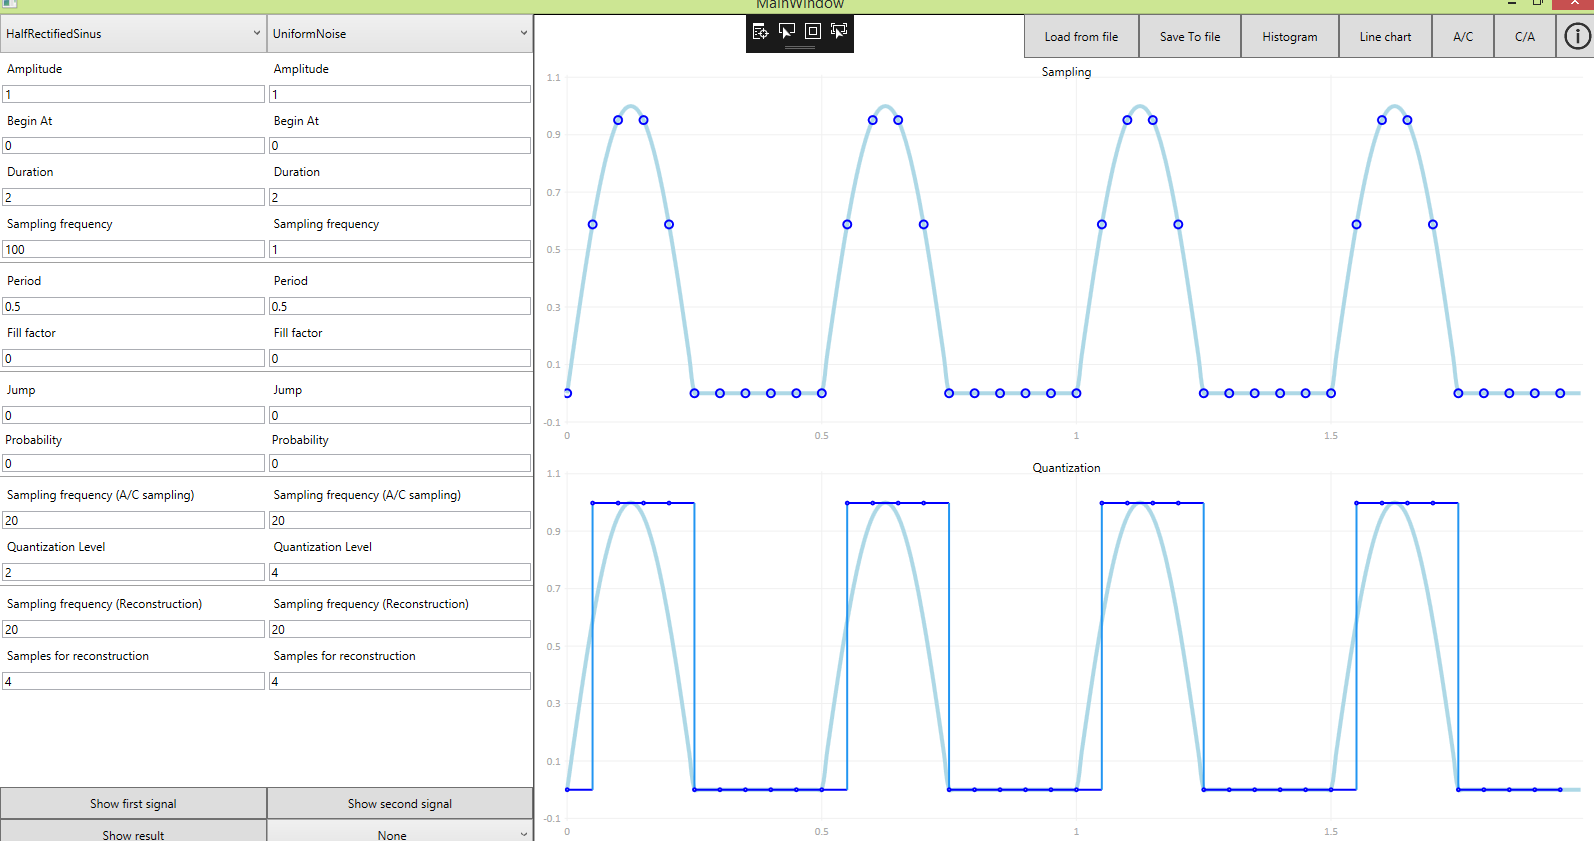
\includegraphics[width=14cm]{images/hsinac1.PNG}
 \vspace{-0.3cm}
 \caption{Konwersja A/C , poziom kwantyzacji = 2}
 \label{gui}
\end{figure}

\begin{figure}[H]
 \centering
 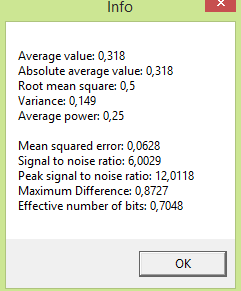
\includegraphics[width=7cm]{images/hsininfo1.PNG}
 \vspace{-0.3cm}
 \caption{Wyliczone wartosci dla sygnału sinusoidalnego wyprostowanego jednopołówkowo  , poziom kwantyzacji = 2}
 \label{gui}
\end{figure}

\begin{figure}[H]
 \centering
 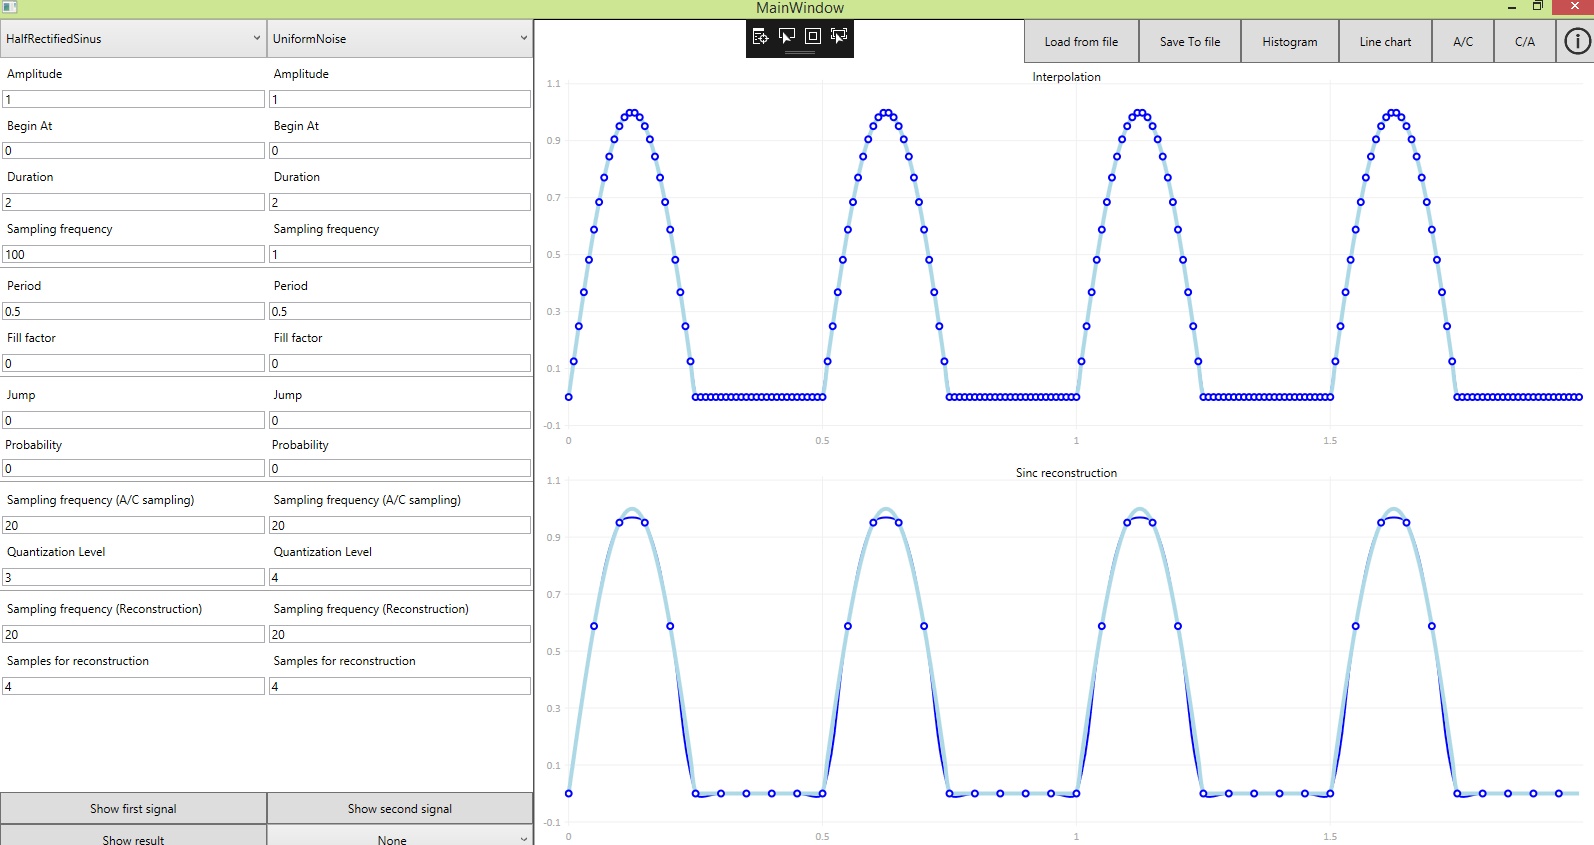
\includegraphics[width=14cm]{images/hsinca.PNG}
 \vspace{-0.3cm}
 \caption{Konwersja C/A}
 \label{gui}
\end{figure}





%%%%%%%%%%%%%%%%%%%%%%%%%%%%%%%%%%%%%%%%%%%%%%%%%%%%%%%%%%%%%%%%%%%%%%%%%%%%%%%%%%%%%%%%%%%%%%%%%%%%%%%%%%%%%%%%%
% PODROZDZIAŁ PT. EKSPERYMENT NR 3
%%%%%%%%%%%%%%%%%%%%%%%%%%%%%%%%%%%%%%%%%%%%%%%%%%%%%%%%%%%%%%%%%%%%%%%%%%%%%%%%%%%%%%%%%%%%%%%%%%%%%%%%%%%%%%%%%


\subsection{Eksperyment nr 3 }
\subsubsection{Różnica sygnału symetrycznego prostokątnego i sygnału sinusoidalnego}
Celem tego eksperymentu było wygenerowanie sygnału będącego różnicą sygnału symetrycznego prostokątnego i sygnału sinusoidalnego


\subsubsection{Rezultat}

\begin{figure}[H]
 \centering
 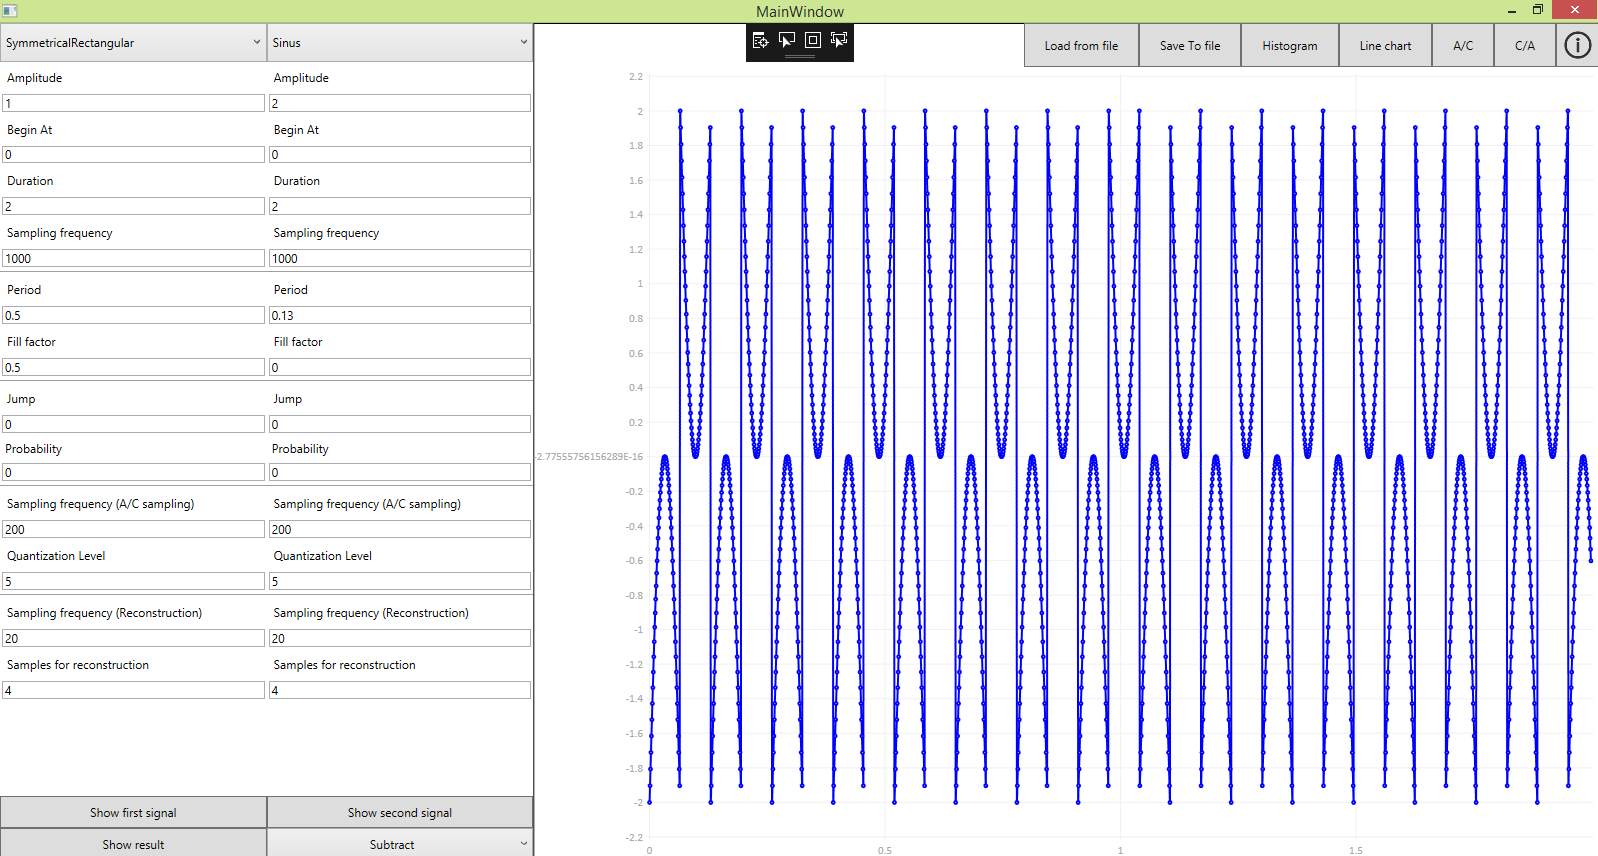
\includegraphics[width=14cm]{images/addline.PNG}
 \vspace{-0.3cm}
 \caption{Wykres różnicy sygnału symetrycznego prostokątnego i sygnału sinusoidalnego}
 \label{gui}
\end{figure}

\begin{figure}[H]
 \centering
 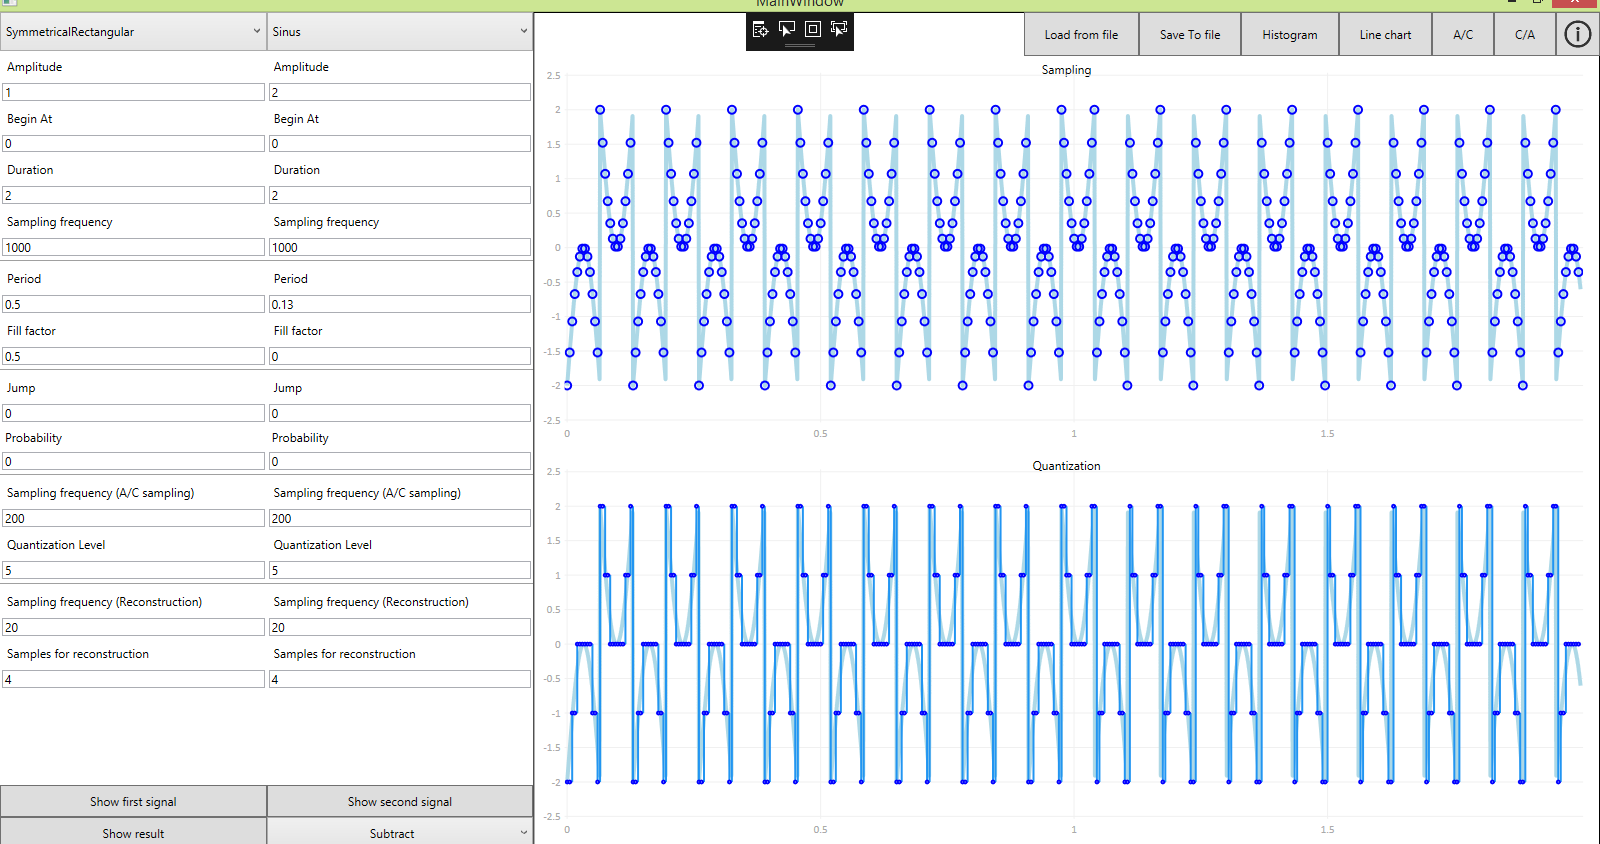
\includegraphics[width=14cm]{images/addac.PNG}
 \vspace{-0.3cm}
 \caption{Konwersja A/C, poziom kwantyzacji = 5}
 \label{gui}
\end{figure}

\begin{figure}[H]
 \centering
 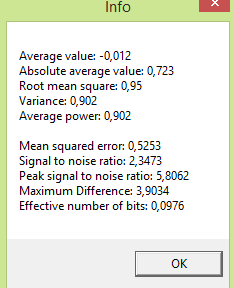
\includegraphics[width=7cm]{images/addinfo.PNG}
 \vspace{-0.3cm}
 \caption{Wyliczone wartosci dla różnicy sygnału symetrycznego prostokątnego i sygnału sinusoidalnego, poziom kwantyzacji = 5}
 \label{gui}
\end{figure}

\begin{figure}[H]
 \centering
 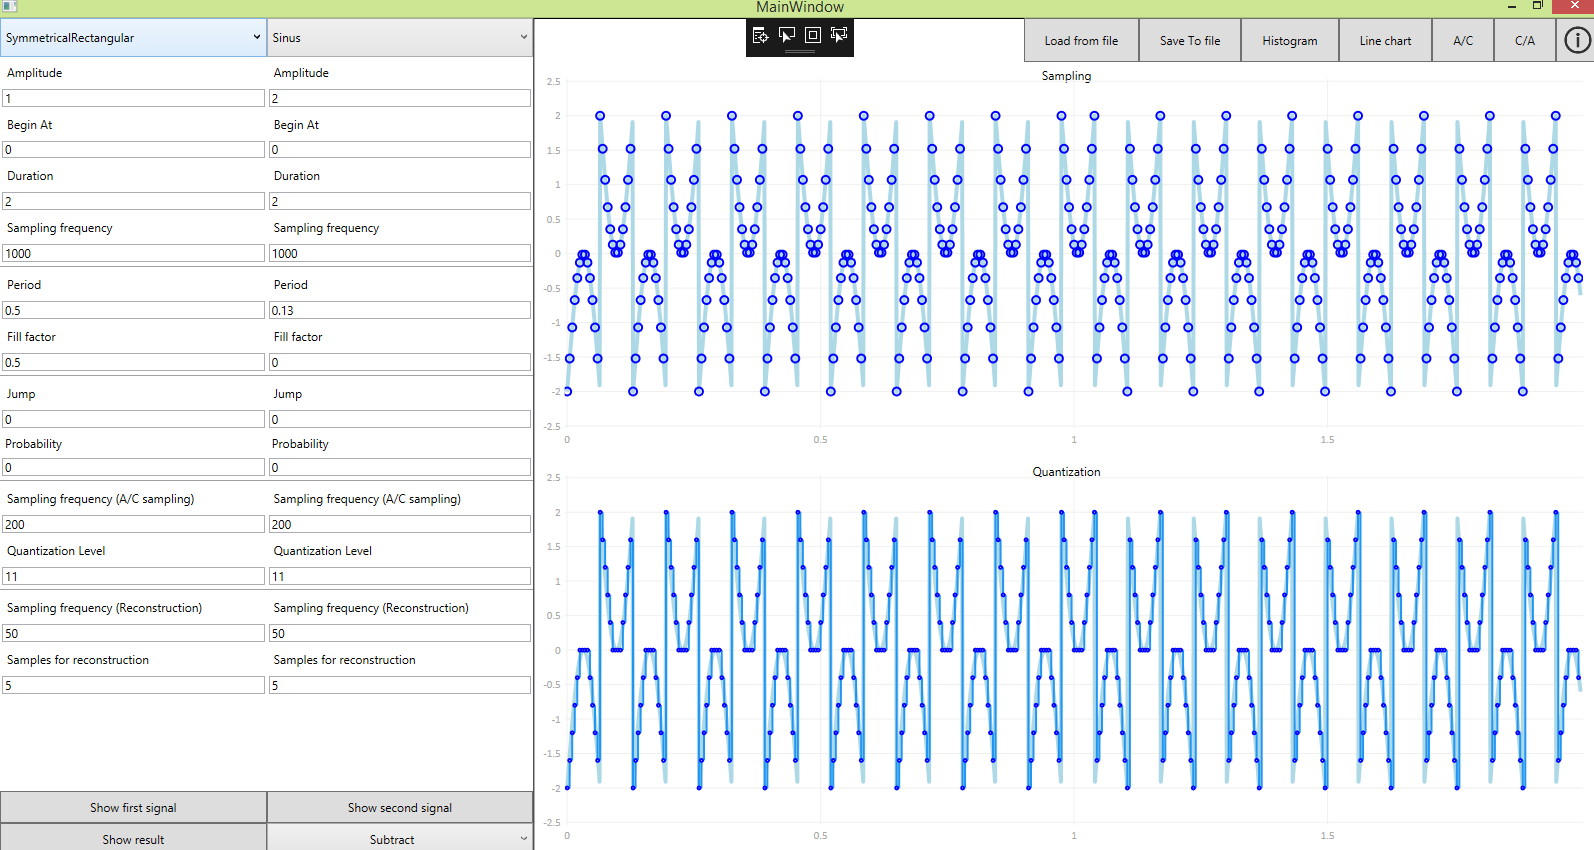
\includegraphics[width=14cm]{images/addac1.PNG}
 \vspace{-0.3cm}
 \caption{Konwersja A/C, poziom kwantyzacji = 11}
 \label{gui}
\end{figure}

\begin{figure}[H]
 \centering
 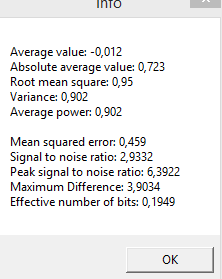
\includegraphics[width=7cm]{images/addacinfo1.PNG}
 \vspace{-0.3cm}
 \caption{Wyliczone wartosci dla różnicy sygnału symetrycznego prostokątnego i sygnału sinusoidalnego, poziom kwantyzacji = 11}
 \label{gui}
\end{figure}

\begin{figure}[H]
 \centering
 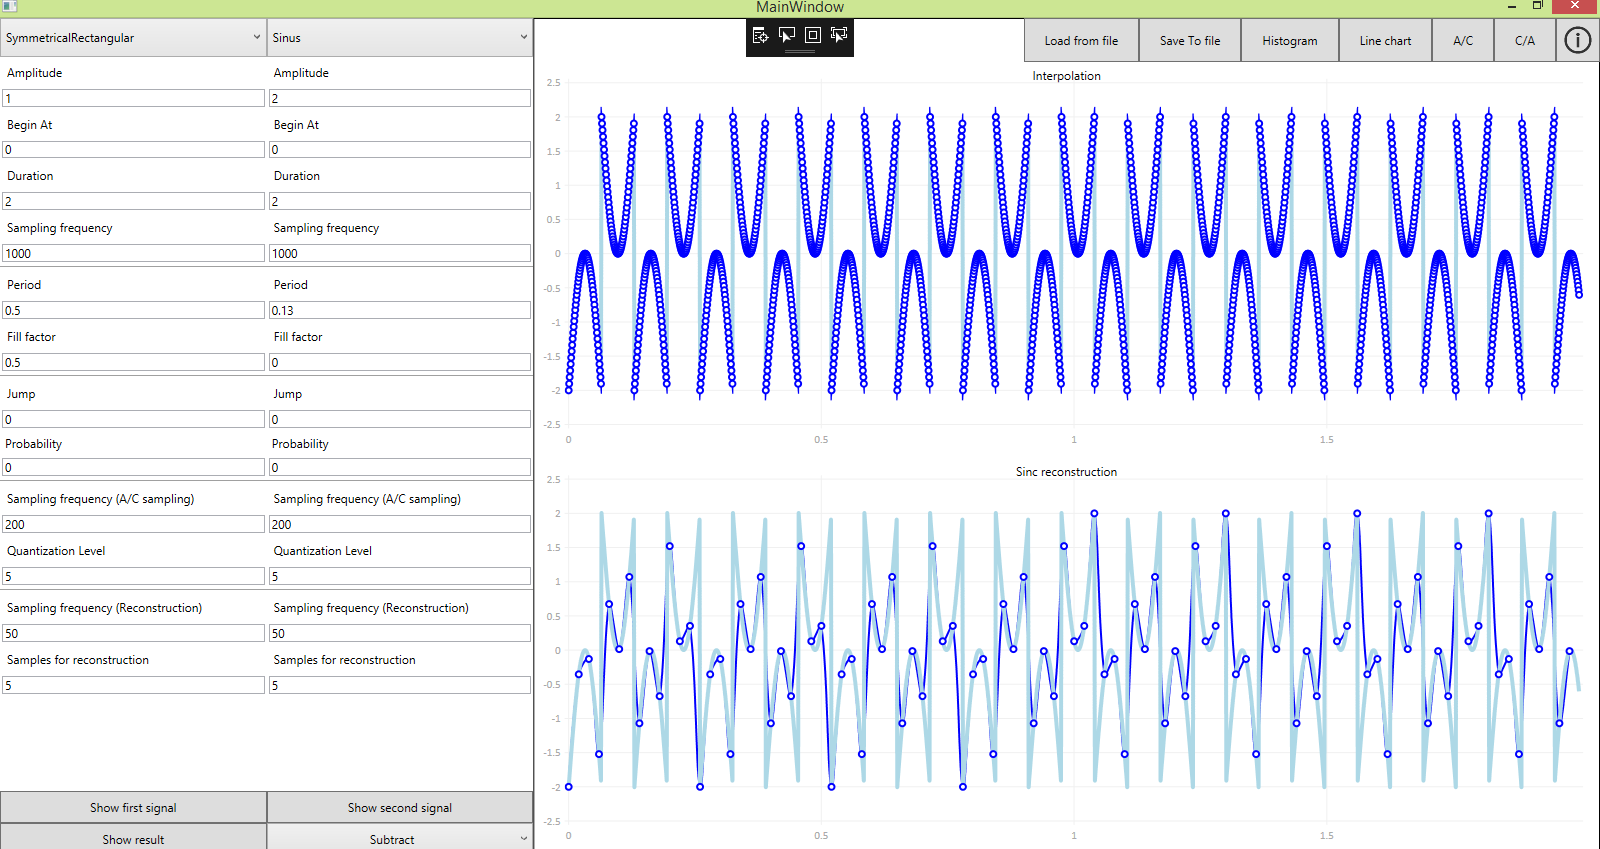
\includegraphics[width=14cm]{images/addca.PNG}
 \vspace{-0.3cm}
 \caption{Konwersja C/A}
 \label{gui}
\end{figure}






\newpage

\section{Wnioski}

Aplikacja została napisania zgodnie z instrukcją zadania \cite{zad}. Aplikacja pozwala na rozszerzanie jej o kolejne funkcjonalnosci na potrzeby kolejnych zadań. 

Dla korelacyjnego czujnika odłegłosci kluczowe jest dobranie odpowiednio dużej częstotliwosci próbkowania, inaczej odległosć jest obliczana z dużym błędem.




%%%%%%%%%%%%%%%%%%%%%%%%%%%%%%%%%%%%%%%%%%%%%%%%%%%%%%%%%%%%%%%%%%%%%%%%%%%%%%%%%%%%%%%%%%%%%%%%%%%%%%%%%%%%%%%%%
% BIBLIOGRAFIA
%%%%%%%%%%%%%%%%%%%%%%%%%%%%%%%%%%%%%%%%%%%%%%%%%%%%%%%%%%%%%%%%%%%%%%%%%%%%%%%%%%%%%%%%%%%%%%%%%%%%%%%%%%%%%%%%%

\begin{thebibliography}{99}
\bibitem{pa} H.~Partl:
\emph{German \TeX},
TUGboat Vol.~9,, No.~1 ('88)
\bibitem{lv} Biblioteka LiveCharts. https://lvcharts.net
\bibitem{wpf} Windows Presentation Foundation. https://docs.microsoft.com/plpl/dotnet/framework/wpf/getting-started/walkthrough-my-frst-wpfdesktop-application
\bibitem{zad} https://ftims.edu.p.lodz.pl/pluginfile.php/13449/mod\_resource/content/0/zadanie3.pdf
\end{thebibliography}

\end{document}
